\section{Технический проект}
\subsection{Общая характеристика организации решения задачи}

Необходимо спроектировать и разработать систему, которая должна выполнять распознавание на основе изображений лиц и отпечатков пальцев с использованием карт пропуска.

Система представляет собой программу, позволяющую пользователю выполнять распознавание лиц и отпечатков пальцев и сканирование карты пропуска для авторизации. Интерфейс включает в себя окно, отображающее видеопоток с камеры и результаты распознавания лица или отпечатка пальца и карты пропуска. Программа автоматически определяет лицо, отпечаток пальца или карту пропуска в кадре, сопоставляет данные и отображает результаты выполнения программы на экране. 

\subsection{Обоснование выбора технологии проектирования}

Используемые для создания интеллектуальной системы языки программирования и технологии соответствуют современным практикам разработки, обеспечивают высокую производительность и отказоустойчивость системы.

\subsubsection{Язык программирования Python}

Язык программирования Python представляет собой высокоуровневый язык общего назначения, отличающийся лаконичным синтаксисом и высокой читаемостью кода. Python обеспечивает возможность реализации объектно-ориентированного, функционального и процедурного стилей программирования. Он обладает мощной стандартной библиотекой, которая охватывает множество областей применения — от работы с файлами и сетями до многопоточности и регулярных выражений. Python широко используется в научных вычислениях, благодаря таким библиотекам как NumPy, SciPy, Pandas и Matplotlib. В области машинного обучения и нейросетей Python является наилучшим языком программирования, благодаря таким инструментам как PyTorch, TensorFlow и Scikit-learn. Кроме того, язык поддерживается большим сообществом, что облегчает поиск решений и развитие проектов.

\subsubsection{Библиотека OpenCV}

OpenCV представляет собой мощную библиотеку компьютерного зрения и обработки изображений, предназначенную для выполнения широкого спектра задач, связанных с анализом изображений и видео. Она предоставляет высокоуровневые и низкоуровневые средства для работы с изображениями, включая функции для обработки, фильтрации, распозна-вания объектов и анализа движения. Основное преимущество OpenCV заключается в её высокой производительности, гибкости и поддержке широкого спектра алгоритмов компьютерного зрения. Благодаря интеграции с языком Python, OpenCV позволяет быстро разрабатывать приложения, связанные с обработкой изображений и видео, и является популярным инструментом как для учебных, так и для полноценных исследовательских и промышленных проектов.

\subsubsection{Библиотека PyTorch}

PyTorch — это современная библиотека машинного и глубокого обучения, предназначенная для создания и обучения нейронных сетей. Она предоставляет интуитивно понятные инструменты для работы с тензорами, автоматического дифференцирования и построения моделей. Одним из ключевых преимуществ PyTorch является использование динамической вычислительной графики, что делает разработку и отладку нейросетей более гибкой и наглядной. Библиотека поддерживает ускорение вычислений с помощью графических процессоров (GPU), что существенно повышает производительность при обучении моделей. Благодаря тесной интеграции с Python, а также множеству встроенных модулей и готовых архитектур, PyTorch широко применяется в задачах компьютерного зрения, обработки естественного языка, биометрии и других областях искусственного интеллекта.

\subsubsection{Библиотека NumPy}

NumPy представляет собой фундаментальную библиотеку для численных вычислений в Python, обеспечивающую поддержку многомерных массивов и высокоуровневых математических операций над ними. Благодаря высокоэффективным операциям с массивами и встроенным линейным алгебраическим методам, NumPy позволяет обрабатывать изображения больших размеров с минимальными затратами ресурсов, что делает её незаменимой в задачах, связанных с сжатием, декомпрессией и преобразованием графических данных.

\subsubsection{Библиотека tkinter}

Для построения графического интерфейса в проекте выбрана библиотека tkinter, которая является частью стандартной поставки Python и представляет собой обёртку над библиотекой Tcl/Tk. Этот выбор объясняется рядом технологических и практических преимуществ:
\begin{enumerate}
	\item Отсутствие необходимости в установке сторонних зависимостей делает tkinter особенно удобным для использования в проектах с упрощённым процессом развёртывания. 
	\item Простота проектирования интерфейса позволяет легко создавать окна, формы, кнопки, меню, вкладки и другие элементы без необходимости изучения сложных графических фреймворков. Это способствует быстрому созданию прототипов и конечных версий интерфейса.
	\item Полная кроссплатформенность интерфейса гарантирует его одинаковое отображение и поведение на всех операционных системах, что избавляет разработчика от необходимости писать отдельные реализации под разные платформы.
	\item Наличие компонентов высокого уровня, таких как текстовые поля, выпадающие списки, кнопки, панели и таблицы, даёт возможность создать функциональный и интуитивно понятный интерфейс для работы с данными.
	\item Возможность динамического обновления интерфейса обеспечивает удобную визуализацию изменений.
\end{enumerate}

tkinter полностью удовлетворяет требованиям к простому, лёгкому в использовании, но функциональному графическому интерфейсу, особенно в условиях ограниченного времени и ресурсов.	

\subsubsection{Библиотека Python Imaging Library}

Python Imaging Library, сокращенно PIL — это библиотека для работы с растровыми изображениями, обеспечивающая поддержку различных форматов, таких как JPEG, PNG, BMP и других. PIL предоставляет широкий набор функций для загрузки, сохранения, обработки и преобразования изображений, что упрощает различные взаимодействия с файлами изображений, такие как сохранение и загрузка изображений, поэтому она является удобным инструментом для предварительной и финальной обработки графических данных.


\subsection{Архитектура программной системы}

На рисунке 3.1 в виде UML-диаграммы представлена архитектура программной системы.

\begin{figure}[H]
	\centering
	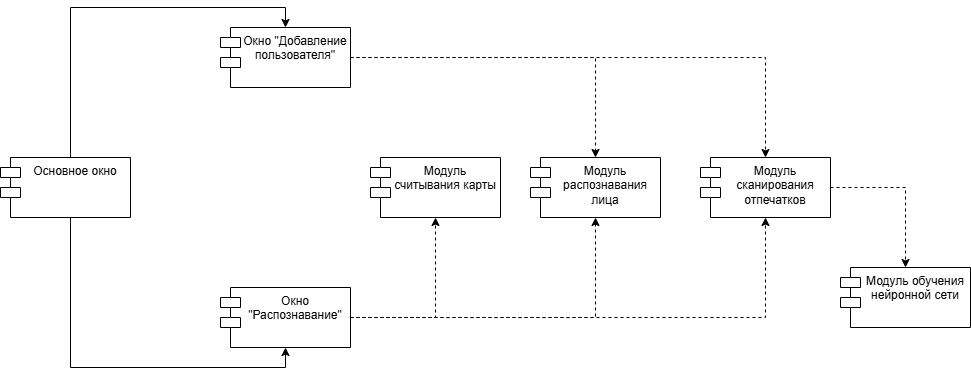
\includegraphics[width=0.7\linewidth]{images/diagramUML}
	\caption{Архитектура системы}
	\label{fig:diagramuml}
\end{figure}

Интеллектуальная система состоит из следующих компонентов:

\begin{enumerate}
	\item Основное окно. Компонент «Основное окно» представляет собой центральный элемент системы, обеспечивающий взаимодействие с пользователем через графический интерфейс. Он отвечает за инициализацию и координацию работы всех подсистем, включая управление потоками и вызовы других модулей для выполнения задач, таких как добавление пользователя или распознавание.
	\item Окно распознавания. Компонент «Окно распознавания» представляет собой специализированный интерфейс, отображающий процесс распознавания пользователя. Он взаимодействует с модулями распознавания лица и сканирования отпечатков, предоставляя пользователю визуальную обратную связь о результатах идентификации.
	\item Окно добавления пользователя. Компонент «Окно добавления пользователя» реализует логику добавления нового пользователя в систему. Он управляет процессом сбора биометрических данных (лица и отпечатков пальцев) и их последующим сохранением в базе данных, обеспечивая интеграцию с модулями захвата и обработки данных.
	\item Модуль считывания карты. Компонент «Модуль считывания карты» отвечает за обнаружение и интерпретацию карт, содержащих идентификационные данные пользователя. Он взаимодействует с камерой для считывания визуальной информации и передает данные в систему для дальнейшей верификации.
	\item Модуль распознавания лица. Компонент «Модуль распознавания лица» предназначен для идентификации пользователя на основе анализа изображений лица, полученных с камеры. Он использует предварительно обученные модели для извлечения векторов и сравнения их с базой данных, обеспечивая точное распознавание. 
	\item Модуль сканирования отпечатков. Компонент «Модуль сканирования отпечатков» реализует функциональность сравнения отпечатков пальцев пользователя с сохраненными в базе данных образцами. Он применяет нейронные сети для анализа биометрических данных и определения степени сходства, что используется в процессе верификации.
	\item Модуль обучения нейронной сети. Компонент «Модуль обучения нейронной сети» отвечает за обучение моделей, используемых для обработки биометрических данных, таких как лица и отпечатки пальцев. Он обеспечивает подготовку и настройку нейронных сетей.
\end{enumerate}

\subsubsection{Архитектура MTCNN}

Нейронная сеть MTCNN представляет собой каскадную систему для обнаружения лиц, состоящую из трёх последовательно работающих сетей: P-Net (сеть предложений), R-Net (сеть уточнения) и O-Net (выходная сеть). 

На рисунке 3.2 изображена структура сети MTCNN.

\begin{figure}[H]
	\centering
	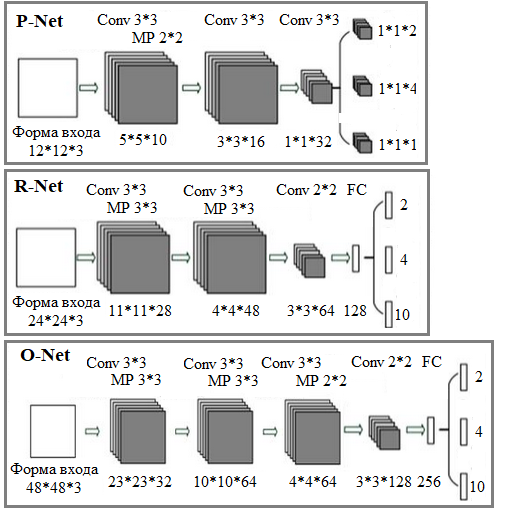
\includegraphics[width=0.7\linewidth]{images/mtcnn}
	\caption{Структура MTCNN}
	\label{fig:mtcnn}
\end{figure}

P-Net — это компактная сеть, которая быстро сканирует изображение и находит возможные места, где могут быть лица. Она работает с изображением, уменьшенным в несколько раз, чтобы учитывать лица разных размеров. Структура сети включает несколько слоёв обработки: сначала изображение проходит через фильтры, выделяющие основные признаки, затем уменьшается в размере, после чего ещё два набора фильтров уточняют анализ. В итоге P-Net выдаёт три результата: вероятность того, что в области есть лицо, координаты рамки вокруг лица и расположение ключевых точек, таких как глаза или рот. Однако эта сеть часто предлагает слишком много вариантов, включая ошибочные, поэтому лишние области отсеиваются специальным методом.

R-Net берёт области, предложенные P-Net, и проверяет их более тщательно, отбрасывая те, где лиц нет, и улучшая рамки вокруг настоящих лиц. Эта сеть сложнее, так как включает дополнительный слой, который объединяет все данные. Она начинает с фильтров, которые выделяют детали, затем уменьшает изображение и применяет ещё несколько фильтров. После этого данные преобразуются в единый набор чисел и анализируются, чтобы определить, есть ли лицо, где оно находится и где расположены ключевые точки. Лишние рамки снова убираются, но с более строгим подходом.

O-Net — финальная сеть, которая делает последний и самый точный анализ. Она работает с более крупными участками изображения, чтобы рассмотреть лицо в деталях. Структура O-Net похожа на R-Net, но включает больше слоёв для обработки данных, что позволяет добиться высокой точности. Она выдаёт окончательные рамки вокруг лиц, вероятность их наличия и координаты ключевых точек.

Общее число параметров MTCNN составляет около 1–2 миллионов, с распределением примерно 10–20 тысяч для P-Net, 100–200 тысяч для R-Net и 300–500 тысяч для O-Net. Сеть предобучена на наборе данных WIDER FACE и используется в системе без дообучения. MTCNN обрабатывает кадры RGB, преобразованные из формата BGR, на устройстве CUDA или CPU.

\subsubsection{Архитектура InceptionResnetV1}

InceptionResnetV1 представляет собой гибридную архитектуру, объединяющую Inception-модули, которые параллельно применяют свёртки разных размеров для извлечения разнообразных признаков, и остаточные соединения, ускоряющие обучение и улучшающие сходимость. Сеть состоит из нескольких ключевых компонентов: начального блока (Stem), Inception-Resnet блоков (A, B, C), блоков уменьшения размерности (Reduction A, B) и финального слоя для создания эмбеддинга. 

На рисунке 3.3 изображена структура сети InceptionResnetV1.

\begin{figure}[H]
	\centering
	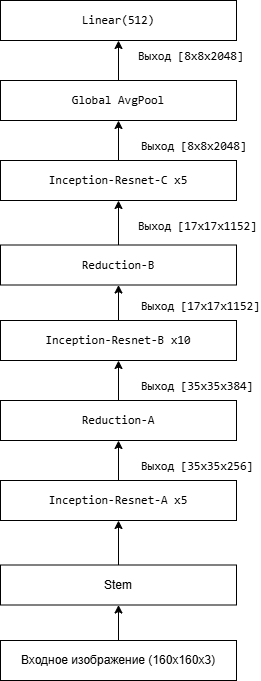
\includegraphics[width=0.3\linewidth]{images/inceptionresnetv1}
	\caption{Структура сети InceptionResnetV1}
	\label{fig:inceptionresnetv1}
\end{figure}


 Работа сети включает в себя следующие этапы:
 
\begin{enumerate}
	\item Предобработка: Изображение лица, вырезанное с помощью MTCNN, масштабируется до 160x160 и нормализуется.
	\item Извлечение признаков: Stem-блок извлекает низкоуровневые признаки (края, текстуры), которые затем обрабатываются Inception-Resnet блоками. Inception-модули параллельно применяют свёртки разных размеров (1x1, 3x3, 7x1 и т.д.), захватывая признаки на разных масштабах. Остаточные соединения ускоряют обучение, добавляя вход блока к его выходу.
	\item Уменьшение размерности: Reduction блоки сокращают пространственные размеры, увеличивая глубину признаков, что позволяет сети фокусироваться на высокоуровневых характеристиках (форма лица, черты).
	\item Генерация векторного представления: Финальный пулинг и полносвязный слой преобразуют признаки в вектор 512D, который используется для сравнения лиц.
\end{enumerate}

Векторные представления сравниваются по косинусному сходству, что определяет, принадлежат ли два изображения одному человеку.

\subsubsection{Архитектура ResNet18}

ResNet18 состоит из начального свёрточного слоя, четырёх блоков остаточных слоёв, глобального усредняющего пулинга и финального слоя. 

На рисунке 3.4 изображена структура сети ResNet18.

\begin{figure}[H]
	\centering
	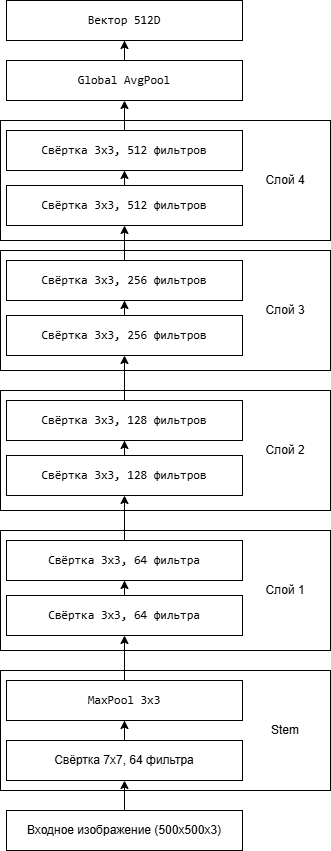
\includegraphics[width=0.3\linewidth]{images/resnet18}
	\caption{Структура сети ResNet18}
	\label{fig:resnet18}
\end{figure}

ResNet18 извлекает признаки из изображения отпечатка пальца, преобразуя его в компактный вектор, который кодирует уникальные характеристики узоров. Процесс включает следующие этапы:

\begin{enumerate}
	\item Предобработка: Изображение отпечатка преобразуется в трёхканальное 500x500 RGB и нормализуется.
	\item Извлечение признаков: Начальный блок извлекает низкоуровневые признаки (края, текстуры). Остаточные блоки (слои 1–4) постепенно увеличивают глубину признаков, уменьшая пространственные размеры. Остаточные соединения добавляют вход модуля к его выходу, упрощая обучение.
	\item Генерация эмбеддинга: После глобального пулинга сеть возвращает вектор 512D, используемый в сиамской нейронной сети.
\end{enumerate}

\subsubsection{Архитектура сиамской нейронной сети}
               
Сиамская нейронная сеть — это архитектура глубокого обучения, разработанная для задач сравнения пар объектов, таких как изображения, с целью определения их сходства или различия. Её ключевая особенность заключается в использовании двух идентичных подсетей с общими весами, которые обрабатывают пару входных данных и создают компактные представления (векторы), сравниваемые с помощью метрики сходства.

На рисунке 3.5 изображена структура сиамской нейронной сети.

\begin{figure}[H]
	\centering
	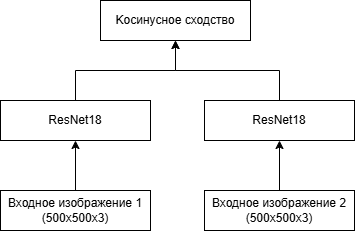
\includegraphics[width=0.6\linewidth]{images/cosine}
	\caption{Структура сиамской нейронной сети}
	\label{fig:cosine}
\end{figure}

Косинусное сходство вычисляется как 

\[
\text{cos}(A,B) = \frac{A \cdot B}{\|A\| \cdot \|B\|} ,
\]

где A, B — векторы 512D. Значение сходства находится в диапазоне [0, 1], и для принятия решения используется порог: если сходство превышает порог, отпечатки считаются принадлежащими одному человеку.

\subsection{Проектирование пользовательского интерфейса}

На основании требований к пользовательскому интерфейсу, представленных в пункте 2.3.3, был разработан графический интерфейс программной системы. 

На рисунке 3.6 представлен макет интерфейса главного окна. Макет содержит следующие элементы:

\begin{enumerate}
	\item Поле для отображения названия программы. 
	\item Кнопка перехода к окну "Добавление пользователя".
	\item Кнопка перехода к окну "Распознавание".
	\item Кнопка выхода из программы.
\end{enumerate}

\begin{figure}[H]
	\centering
	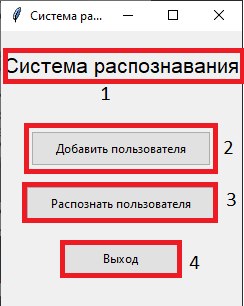
\includegraphics[width=0.4\linewidth]{images/maket2}
	\caption{Макет основного окна}
	\label{fig:maket2}
\end{figure}

На рисунке 3.7 представлен макет интерфейса окна "Распознавание". Макет содержит следующие элементы:

\begin{enumerate}
	\item Поле для отображения вывода с камеры.
	\item Кнопка перехода к главному окну.
\end{enumerate}

\begin{figure}[H]
	\centering
	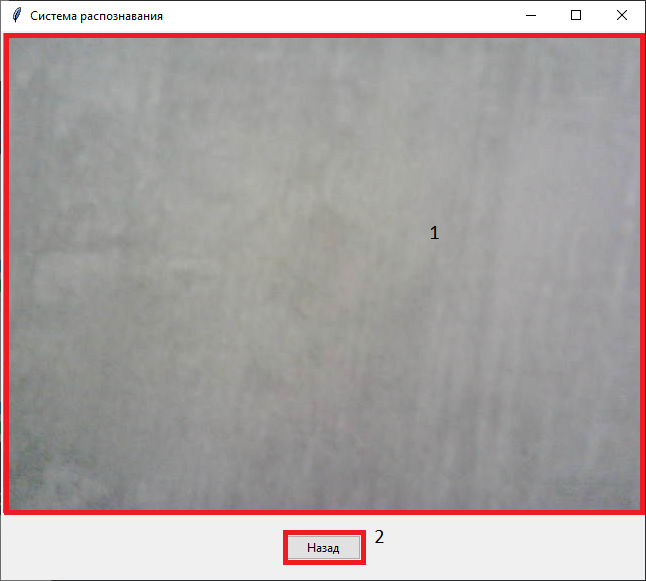
\includegraphics[width=0.7\linewidth]{images/maket3}
	\caption{Макет окна "Распознавание"}
	\label{fig:maket3}
\end{figure}

На рисунке 3.8 представлен макет интерфейса окна "Добавление пользователя". Макет содержит следующие элементы:

\begin{enumerate}
	\item Поле для отображения текста с указаниями. 
	\item Поля для ввода имени пользователя.
	\item Кнопка для запуска сканирования лица.
	\item Кнопка для запуска сканирования отпечатка пальца.
	\item Кнопка для создания карты доступа.
	\item Кнопка выхода из программы.
\end{enumerate}

\begin{figure}[H]
	\centering
	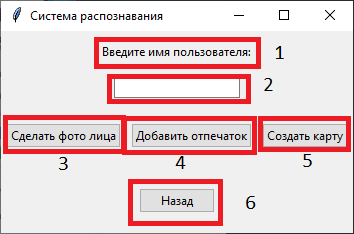
\includegraphics[width=0.7\linewidth]{images/maket1}
	\caption{Макет окна "Добавление пользователя"}
	\label{fig:maket1}
\end{figure}

\newpage